% Set title page for separate titlepage
\documentclass{article}

% Some standard math packages
\usepackage{amsmath}
\usepackage{amssymb}
\usepackage{amsfonts}
\usepackage{pdfpages}
% Package for lists
\usepackage[shortlabels]{enumitem}
% Dashed text
\usepackage{arydshln}
\usepackage[normalem]{ulem}
%rotate page
\usepackage{pdflscape}
% Graphics
\usepackage{tikz}
\usepackage{rotating}
\usepackage{geometry}
\usepackage{pgfgantt}

%Colors
\definecolor{lightblue}{HTML}{4FC3F7}
\definecolor{lightgreen}{HTML}{81C784}
\definecolor{lightorange}{HTML}{FF8A65}

\title{Project monitoring}
%\subtitle{MSc in Computer Science \\ For entry in 2018}

%\author{Luca Dolfi}
\pagestyle{headings}
\markright{Luca Dolfi\hfill \today \hfill}
\begin{document}
%\maketitle
\part*{Project monitoring - version 5}
Each task, at least in the first two milestones, is composed mostly readings and papers review.
At the end of each tasks a small summary will be produced for that task. 
At the end of the milestone all summaries will come together to form a chapter of the final report. \\

\paragraph*{Milestones}
\begin{enumerate}[A)]
\item \sout{Project assessment} COMPLETE 
\item \sout{Concepts of QM} COMPLETE
\item Concepts of information theory
\item Investigation into bound information / Final submission
\end{enumerate}

\centerline{
	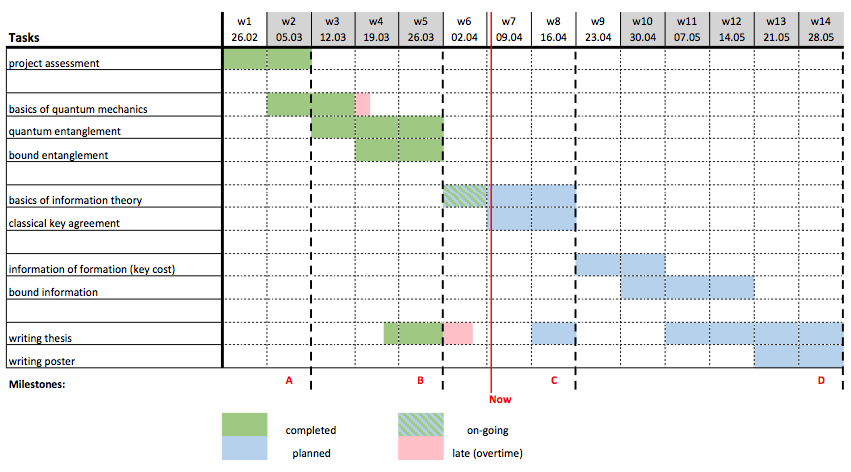
\includegraphics[scale=0.5]{gantt-5.png}
}
\pagebreak
%\begin{sidewaysfigure}
%
%	\begin{ganttchart}[
%	  hgrid,
%	  vgrid,
%	  bar/.append style={fill=lightblue},
%	  vrule/.style={thick,lightgreen},
%	  % Today
%	  today=9,
%	  progress=today,
%	  progress label text={\pgfmathprintnumber[precision=0, verbatim]{#1}\%},
%	  today rule/.style={lightorange, ultra thick},
%	  % Grid vertical size
%	  y unit title=1cm,
%	  y unit chart=0.8cm,
%	  % Grid horizontal size
%	  x unit=0.6cm,
%	]{1}{28}
%	
%	% Top
%	\gantttitle{Spring semester 2018}{28} \ganttnewline
%	\gantttitlelist{1,...,14}{3} \\
%	
%	% Tasks
%	\ganttgroup{Milestone 1: Project Assessment}{1}{6} \ganttnewline
%	\ganttbar{project assessment}{1}{6} \ganttnewline
%	
%	\ganttgroup{Milestone 2: Concepts of QM}{1}{14} \ganttnewline
%	\ganttbar{basics of quantum mechanics}{1}{4} \ganttnewline
%	\ganttbar{quantum entanglement}{8}{12} \ganttnewline
%	\ganttbar{bound entanglement}{8}{12} \ganttnewline
%	
%	\ganttgroup{Milestone 3: Concepts of information theory}{13}{24} \ganttnewline
%	\ganttbar{basics of information theory}{13}{18} \ganttnewline
%	\ganttbar{classical key agreement}{17}{22} \ganttnewline
%	
%	\ganttgroup{Milestone 4: Investigation into bound information / Final submission}{10}{28} \ganttnewline
%	\ganttbar{Write thesis}{10}{10}
%		\ganttbar{}{15}{16}
%		\ganttbar{}{19}{20} \ganttnewline
%	\ganttbar{Create poster, write report}{23}{28} \ganttnewline
%	
%	% Milestones
%	\ganttvrule{M1}{10}
%	\ganttvrule{M2}{14}
%	\ganttvrule{M3}{24}
%	\ganttvrule{M4}{28}
%	
%	\end{ganttchart}
%
%\end{sidewaysfigure}
\end{document}
